%===================================================================================
% JORNADA CIENTÍFICA ESTUDIANTIL - MATCOM, UH
%===================================================================================
% Esta plantilla ha sido diseñada para ser usada en los artículos de la
% Jornada Científica Estudiantil de MatCom.
%
% Por favor, siga las instrucciones de esta plantilla y rellene en las secciones
% correspondientes.
%
% NOTA: Necesitará el archivo 'jcematcom.sty' en la misma carpeta donde esté este
%       archivo para poder utilizar esta plantila.
%===================================================================================



%===================================================================================
% PREÁMBULO
%-----------------------------------------------------------------------------------
\documentclass[a4paper,10pt,twocolumn]{article}

%===================================================================================
% Paquetes
%-----------------------------------------------------------------------------------
\usepackage{amsmath}
\usepackage{amsfonts}
\usepackage{amssymb}
\usepackage{jcematcom}
\usepackage[utf8]{inputenc}
\usepackage{listings}
\usepackage[pdftex]{hyperref}
\usepackage{caption}
\usepackage{subcaption}
%-----------------------------------------------------------------------------------
% Configuración
%-----------------------------------------------------------------------------------
\hypersetup{colorlinks,%
	    citecolor=black,%
	    filecolor=black,%
	    linkcolor=black,%
	    urlcolor=blue}

%===================================================================================



%===================================================================================
% Presentacion
%-----------------------------------------------------------------------------------
% Título
%-----------------------------------------------------------------------------------
\title{Proyecto de Modelos de Matemática Aplicada. \\Construcción y graficación de grafos causales}

%-----------------------------------------------------------------------------------
% Autores
%-----------------------------------------------------------------------------------
\author{\\
\name Dennis Fiallo Muñoz \email \href{mailto: dennis.fiallo@estudiantes.matcom.uh.cu}{dennis.fiallo@estudiantes.matcom.uh.cu}
	\\ \addr Grupo C-311 \AND
\name Lauren O. Guerra Herández \email \href{mailto:lauren.guerra@estudiantes.matcom.uh.cu}{lauren.guerra@estudiantes.matcom.uh.cu}
  \\ \addr Grupo C-312}

%-----------------------------------------------------------------------------------
% Tutores
%-----------------------------------------------------------------------------------
\tutors{\\
Dr. Ferando Rodríguez Flores \emph{MatCom} \\
Lic. Ania , \emph{MatCom}}

%-----------------------------------------------------------------------------------
% Headings
%-----------------------------------------------------------------------------------
\jcematcomheading{\the\year}{1-\pageref{end}}{D. Fiallo, L. Guerra}

%-----------------------------------------------------------------------------------
\ShortHeadings{Ejemplo JCE}{Autores}
%===================================================================================



%===================================================================================
% DOCUMENTO
%-----------------------------------------------------------------------------------
\begin{document}

%-----------------------------------------------------------------------------------
% NO BORRAR ESTA LINEA!
%-----------------------------------------------------------------------------------
\twocolumn[
%-----------------------------------------------------------------------------------

\maketitle

%===================================================================================
% Resumen y Abstract
%-----------------------------------------------------------------------------------
\selectlanguage{spanish} % Para producir el documento en Español

%-----------------------------------------------------------------------------------
% Resumen en Español
%-----------------------------------------------------------------------------------
\begin{abstract}

	Se necesita para investigaciones en el Centro de Neurociencias de Cuba una aplicación que ayude a los investigadore a representar en forma de grafo las de conexiones causales en el cerebro humano Hacer un programa al cual se le pasen dos tensores de conectividad y una lista con los nombres de los nodos y construir un grafo como se explicó anteriormente que admita las 360 necesarias y se puedan ver correctamente los nodo, las conexiones y la fuerza de estas.


\end{abstract}

%-----------------------------------------------------------------------------------
% English Abstract
%-----------------------------------------------------------------------------------
\vspace{0.5cm}

\begin{enabstract}

  The English abstract must have have $100$ to $200$ words, and present 
  the essentials of the article content in a clear and concise form.

\end{enabstract}

%-----------------------------------------------------------------------------------
% Palabras clave
%-----------------------------------------------------------------------------------
\begin{keywords}
	grafos causales,
	librerías,
	python
\end{keywords}

%-----------------------------------------------------------------------------------
% Temas
%-----------------------------------------------------------------------------------
%\begin{topics}
%	Tema, Subtema.
%\end{topics}


%-----------------------------------------------------------------------------------
% NO BORRAR ESTAS LINEAS!
%-----------------------------------------------------------------------------------
\vspace{0.8cm}
]
%-----------------------------------------------------------------------------------


%===================================================================================

%===================================================================================
% Introducción
%-----------------------------------------------------------------------------------
\section{Introducción}\label{sec:intro}
%-----------------------------------------------------------------------------------

Se necesita para investigaciones en el Centro de Neurociencias de Cuba una aplicación que ayude a los investigadore a representar en forma de grafo las de conexiones causales y contemporánea que ocurren en el cerebro humano para esto nos proponemos hacer un programa al cual se le pasen dos tensores de conectividad y una lista con los nombres de los nodos y con estos datos construir un grafo que admita las 360 conexiones necesitadas y además se vea de la mejor manera posible para apoyar su estudio y análisis.\\

El proceso de contrucción de grafo causales se realiza a partir de dos tensores de 360x360xlags, siendo uno binario indicando si hubo conexión o no, y otro de pesos indicando la fuerza de las conexiones. Estos se construyen de la siguiente manera:

\begin{description}


\item	Conexiones contemporáneas: Se representan con una línea recta. Se toma el lag 0(único lag simétrico) y donde aparezca 1 significa que hay conexión entre los nodos (i, j), mientras que el color de la conexión que se traza viene dado por el valor de la matriz de peso en la posición (i, j).\\

\item	Lagged connections o causalidad: Se representan con flechas. Para el resto de lags se busca igualmente si hay un 1 en el tensor binario de 
lag$\neq $0 y se construye una flecha del nodo i al j con la intensidad dada por el promedio de los valores de la matriz de pesos en los lags donde hubo conexión, además de especificar los lags con conexión.\\

\end{description}

\begin{figure}[h!]%
\center
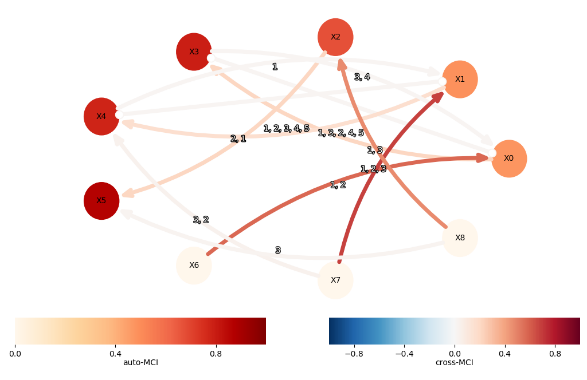
\includegraphics[scale=0.95]{example1.png}
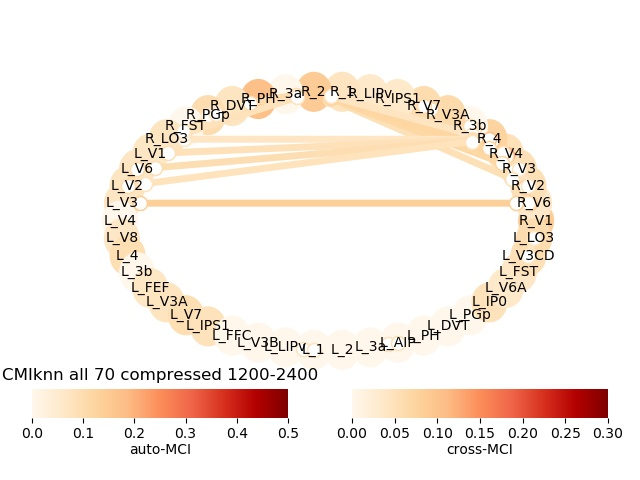
\includegraphics[scale=0.45]{example.png}
\caption{Ejemplo de graficación de grafos causales que se pueden ver con precisión}
\end{figure}

\newpage


Las aplicaciones con las que cuenta el usuario al pasarle un gráfico de más de 180 series de tiempo(en la práctica se necesitan 360), el programa pone 180 nodos sobre una circunferencia y los restantes los sobrepone a estos en la misma circunferencia, haciendo que no sea posible ver las conexiones.\\


\begin{figure}[h!]%
\center
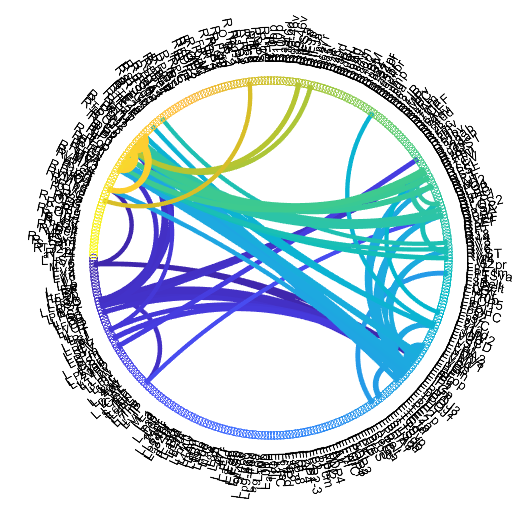
\includegraphics[scale=0.3]{example2.png}
\caption{Ejemplo de graficación en que los nodos se superponen y no se pueden observar los resultados}
\end{figure}
 
 
Por esto nuestro objetivo es hacer un programa al cual se le pasen dos tensores de conectividad y una lista con los nombres de los nodos y construir un grafo como se explicó anteriormente que admita las 360 necesarias y en general la cantidad de conexiones que se necesiten representar en cada caso y se puedan ver correctamente los nodo, las conexiones y la fuerza de estas. \\

También otro problema que presenta el usuario es que guarda cada uno de los pares de tensores que se utilizan para la contrucción de los grafos en formato matlab, donde cada archivo .mat que contiene un par de tensores ocupa un espacio de más de 3.0 mb, por lo cual al tener cientos de archivos de este tipo para su investigación ocupan un espacio considerable, por esto además nos propusimos que una vez conformado el grafo, sea guardado en un archivo que pese mucho menos y luego este pueda ser cargado desde nuestra misma aplicación. 

\section*{Primeras ideas}

Al comienzo de la realización de este proyecto se tenía en mente la implementación de métodos para dibujar grafos que lograran una buena ditribución de nodos y aristas en el espacio bidimensional utilizando los conocimientos adquiridos en asignaturas como Matemática Discreta II, Estructura de Datos y Algoritmos II y Modelos de Optimización, esto dibujando el grafo en su forma maximal planar y luego ir añadiendo las aristas que falten por dibujarse  minimizando la cantidad de aristas que serían dibujadas cortando a las que ya estuvieran colocadas. \\

Esto tuvo grandes inconvenientes porque los grafo causales están muy lejos de ser planares, tienen muchas aristas y a la hora de acomodar los nodos y dibujar las aristas que no formaban parte del grafo maximal planar tomado como base no se podían garantizar distrubuciones de nodos y aristas que garantizaran la correcta observación del grafo.\\

Buscando en el estado del arte no existía nada como esto, ninguna distribución que se hiciera a un grafo resultaba buena en todos los casos, para todo tipo de grafos, probamos con la librería networkx las diferentes distribuciones que esta tiene implementadas y ninguna de ellas cumplía nuestro objetivo, por lo que llegamos a la conclusión que crear un algoritmo que graficara cualquier grafo de la mejor manera poible para él es un ejercicio muy complicado por lo cual no se encontraba a nuestro alcance.\\

Por esto nos propusimos utilizar las mejores implementaciones de dibujo de grafos que estuvieran disponibles en librerías de python para poder resolver el problema del usuario y lograr su satisfacción y comodidad.\\


\section*{Solución}













%===================================================================================



%-----------------------------------------------------------------------------------
	\subsection{Listas y Descripciones}\label{sub:lists}
%-----------------------------------------------------------------------------------
		Para producir listas enumeradas, utilice el siguiente estilo:
		\begin{enumerate}
			\item Primer Elemento
			\item Segundo Elemento
			%
			\begin {enumerate}
				\item {Segundo Elemento - Subítem Uno}
				\item {Segundo Elemento - Subítem Dos}
			\end {enumerate}
			%
		\end{enumerate}

%-----------------------------------------------------------------------------------
		Para producir descripciones, use el siguiente estilo:

%-----------------------------------------------------------------------------------
		\begin{description}
			\item [Primer Elemento] con su respectiva descripción.
			\item [Segundo Elemento] también con su respectiva descripción.
		\end{description}

%-----------------------------------------------------------------------------------
	\subsection{Figuras}\label{sub:figures}
%-----------------------------------------------------------------------------------
		Para producir cuerpos flotantes (figuras o tablas), asegúrese de numerar
		y etiquetar correctamente cada figura. Las referencias a las figuras deben
		estar correctamente etiquetadas. Por ejemplo, véase la Fig. \ref{fig:ex}\ldots

		\begin{figure}[h!]%
		\begin{center}
			\begin{tabular}{|c|c|c|} \hline
			 			& Método 1 	& Método 2 	\\ \hline
			A 			&  			&  			\\ \hline
			B			& 			& 			\\ \hline
			C 			& 			&  			\\ \hline
			\end{tabular}
		\caption{Figura de ejemplo. Recuerde especificar el origen de los datos que se muestran. \label{fig:ex}}
		\end{center}
		\end{figure}

%-----------------------------------------------------------------------------------
	\subsection{Código Fuente}\label{sub:listings}
%-----------------------------------------------------------------------------------
		Para producir código fuente, envuélvalo en una figura flotante y
		etiquételo correctamente. Por ejemplo, en la Fig. \ref{fig:code}
		se muestra un código bastante conocido\ldots

		% Configuración de Listings
		\lstset{keywordstyle=\color{blue}, basicstyle=\small}

		\begin{figure}[htb]%
			\begin{lstlisting}[language=c]%

    int main(int argc, char** argv)
    {
        // Imprimiendo "Hola Mundo".
        printf("Hello, World");
    }

			\end{lstlisting}
		\caption{Código fuente de ejemplo.\label{fig:code}}
		\end{figure}

%-----------------------------------------------------------------------------------
	\subsection{Referencias}
%-----------------------------------------------------------------------------------
  	Las referencias deben estar agrupadas en una sección al final del artículo,
  	y las citas numeradas correctamente, por ejemplo \cite{knuth} o \cite{goedel}.
  	Incluya toda la información importante de cada referencia, incluídos autor,
  	título, y notas de la edición. En caso de citar sitios web, además
  	de la URL, incluya la fecha en que fue consultado, como en \cite{wiki}. Numere 
  	las referencias según el orden en que se les cita.

%===================================================================================



%===================================================================================
% Conclusiones
%-----------------------------------------------------------------------------------
\section{Conclusiones}\label{sec:conc}

  En esta sección puede incluir las conclusiones de su investigación y las ideas
  sobre la continuidad del trabajo, en el caso que aplique.

%===================================================================================



%===================================================================================
% Recomendaciones
%-----------------------------------------------------------------------------------
\section{Recomendaciones}\label{sec:rec}

  En esta sección puede incluir recomendaciones sobre posibles formas de continuar
  la investigación u otros temas relacionados.

%===================================================================================



%===================================================================================
% Bibliografía
%-----------------------------------------------------------------------------------
\begin{thebibliography}{99}
%-----------------------------------------------------------------------------------
	\bibitem{knuth} Donald E. Knuth. \emph{The Art of Computer Programming}.
		Volume 1: Fundamental Algorithms (3rd~edition), 1997.
		Addison-Wesley Professional.

	\bibitem{goedel} Kurt Göedel. \emph{Über formal unentscheidbare Sätze der
		Principia Mathematica und verwandter Systeme, I}.
		Monatshefte für Mathematik und Physik 38.

	\bibitem{wiki} Wikipedia. URL: \href{http://en.wikipedia.org}
	  {http://en.wikipedia.org}.
		Consultado en \today.

%-----------------------------------------------------------------------------------
\end{thebibliography}

%-----------------------------------------------------------------------------------

\label{end}

\end{document}

%===================================================================================
